 %% ----------------------------------------------------------------
%% Thesis.tex -- MAIN FILE (the one that you compile with LaTeX)
%% ---------------------------------------------------------------- 

% Set up the document
\documentclass[a4paper, 11pt, oneside]{thesis}  % Use the "Thesis" style, based on the ECS Thesis style by Steve Gunn
\graphicspath{{Figures/}}  % Location of the graphics files (set up for graphics to be in PDF format)

%Abbreviations
\usepackage{enumitem}
\newlist{abbrv}{itemize}{1}
\setlist[abbrv,1]{label=,labelwidth=1in,align=parleft,itemsep=0.1\baselineskip,leftmargin=!}

\usepackage{datatool}
\newcommand{\sortitem}[2][\relax]{%
  \DTLnewrow{list}% Create a new entry
  \ifx#1\relax
    \DTLnewdbentry{list}{sortlabel}{#2}% Add entry sortlabel (no optional argument)
  \else
    \DTLnewdbentry{list}{sortlabel}{#1}% Add entry sortlabel (optional argument)
  \fi%
  \DTLnewdbentry{list}{description}{#2}% Add entry description
}
\newenvironment{abbrvsorted}{%
  \DTLifdbexists{list}{\DTLcleardb{list}}{\DTLnewdb{list}}% Create new/discard old list
}{%
  \DTLsort{description}{list}% Sort list
  \begin{abbrv}%
    \DTLforeach*{list}{\theLabel=sortlabel, \theDesc=description}{%
      \item[\theLabel] \theDesc}% Print each item
  \end{abbrv}%
}

\newenvironment{abbreviations}{%
  \DTLifdbexists{list}{\DTLcleardb{list}}{\DTLnewdb{list}}% Create new/discard old list
}{%
%  \DTLsort{description}{list}% Sort list
  \begin{abbrv}%
    \DTLforeach*{list}{\theLabel=sortlabel, \theDesc=description}{%
      \item[\theLabel] \theDesc}% Print each item
  \end{abbrv}%
}


% Include any extra LaTeX packages required
\usepackage[square, numbers, comma, sort&compress]{natbib} 	 % Use the "Natbib" style for the references in the Bibliography
\usepackage{verbatim}  % Needed for the "comment" environment to make LaTeX comments
\usepackage{vector}  % Allows "\bvec{}" and "\buvec{}" for "blackboard" style bold vectors in maths
\hypersetup{urlcolor=blue, colorlinks=true}  % Colours hyperlinks in blue, but this can be distracting if there are many links.
%\usepackage[ruled]{algorithm2e}
%\renewcommand{\algorithmcfname}{ALGORITHM}
% Langue
\usepackage[T1]{fontenc}
\usepackage[mac]{inputenc}
\usepackage[frenchb,english]{babel} % On peut aussi mettre english ici.
% Figures et couleurs
\usepackage{graphicx}
\usepackage{subfigure}
\usepackage{color}
\definecolor{gris}{gray}{0.45}
\usepackage{appendix}
\usepackage{MnSymbol}
\usepackage{multirow}
\usepackage{listings}
\usepackage{algorithm}
\usepackage{algpseudocode}
% Font math
\usepackage{hyperref}
\usepackage{amssymb, amsmath, amsfonts} 
\usepackage{dsfont}
% Mise en page latex et police
\usepackage{vmargin}
\usepackage{tikz-timing}[2009/05/15]
\usepackage{tikz}
\usetikzlibrary{shapes,arrows,shadows}
\usepackage{verbatim}
\usetikzlibrary[patterns]
\usepackage[underline=true,rounded corners=false]{pgf-umlsd}
\usepackage{setspace}
\usepackage{enumerate}
%\doublespace
%\setlength{\parskip}{2cm}
%\setlength{\baselineskip}{2cm plus 0pt minus 0pt}
\usepackage{pdfpages}
\usepackage{epsfig}

% New command
\newcommand{\maxdmin}{\mbox{$\max\!\text{-}d_{\min}$}}
\newcommand{\maxlmin}{\mbox{$\max\!\text{-}\lambda_{\min}$}}
\newcommand{\dmin}{$d_{\min}$}

\DeclareMathOperator*{\argmax}{arg\,max}
\DeclareMathOperator*{\argmin}{arg\,min}
\DeclareMathOperator{\cotan}{cotan}
\DeclareMathOperator{\atan}{atan}
\DeclareMathOperator{\rank}{rank}
\DeclareMathOperator{\diag}{diag}
\DeclareMathOperator{\trace}{trace}

\newcommand{\blankspace}{\clearpage
\thispagestyle{empty}
\phantom{a}
\vfill
\newpage
\vfill
\addtocounter{page}{-1}} 

%% ----------------------------------------------------------------
\begin{document}
%\setlength{\baselineskip}{2cm plus 0pt minus 0pt}

%\newlength{\plarg}
%\setlength{\plarg}{8cm}
%\newlength{\glarg}
%\setlength{\glarg}{14cm}
%\newlength{\Glarg}
%\setlength{\Glarg}{15cm}
%


%\includepdf[offset= 80 -80]{couverture-latex.pdf}



%\blankspace
\frontmatter	  % Begin Roman style (i, ii, iii, iv...) page numbering

\setcounter{page}{1}
\pagenumbering{Roman}

% Set up the Title Page
\title  {FTA-MAC}
\authors  {\texorpdfstring
            {\href{van-thiep.nguyen@irisa.fr}{Van-Thiep NGUYEN}}
            {Van-Thiep NGUYEN}
            }
\addresses  {\groupname\\\deptname\\\univname}  % Do not change this here, instead these must be set in the "Thesis.cls" file, please look through it instead
\date   {\today}
\subject    {}
\keywords   {}

%\maketitle
% ----------------------------------------------------------------

\setstretch{1.3}  % It is better to have smaller font and larger line spacing than the other way round

% Define the page headers using the FancyHdr package and set up for one-sided printing
\fancyhead{}  % Clears all page headers and footers
\rhead{\thepage}  % Sets the right side header to show the page number
\lhead{}  % Clears the left side page header

\pagestyle{fancy}  % Finally, use the "fancy" page style to implement the FancyHdr headers

%\addtocounter{page}{-1} % Pour revenir a 0 dans la numerotation des pages.

%%%%%%%%%%
% PREMIERE DE COUVERTURE
%%%%%%%%%%

\newlength{\plarg}
\setlength{\plarg}{8cm}
\newlength{\glarg}
\setlength{\glarg}{14cm}
\newlength{\Glarg}
\setlength{\Glarg}{15cm}

\begin{titlepage}
\thispagestyle{empty}
%\noindent
%\noindent
%\begin{minipage}{\glarg}
%{\large LOGO labo} \hfill {\large LOGO Ecole} 
%{\rule{\glarg}{1pt}} \vspace{-1cm}
%\begin{center}
%\begin{tabular}{p{13cm}r}
%\hspace{-2mm}\textbf{Nom Labo} & \textbf{LABO} \\
%\hspace{-2mm}Nom complet & Section \dots \\
%\hspace{-2mm}du laboratoire & 
%\end{tabular}
%\end{center}
%\end{minipage}

\vspace{-1cm}
\begin{minipage}{\glarg}
\vspace{-4.5cm}
\hspace{-1.5cm}{\color{gris}\large\bf N$^o$ d'ordre  : \hspace{9.5cm} \bf ANN\'EE 2016}
\end{minipage}
\vspace{-2cm}
\begin{figure}[htp]
\center
\hspace{-1cm}
\includegraphics[angle=0,width=16cm]{Logos.png}
\end{figure}

\begin{center}
\begin{minipage}{\glarg}
\vspace{0.5cm}
\centering{\Large\bfseries TH\`ESE / UNIVERSIT\'E DE RENNES 1}\\ \vspace{0mm}\emph{\Large sous le sceau de l'Universit\'e Europ\'eenne de Bretagne}\\ \vspace{0.5cm}
{\Large pour le grade de}\\ \vspace{2mm}
{\Large\bf DOCTEUR DE L'UNIVERSIT\'E DE RENNES 1}\\ \vspace{0.4cm}
\emph{\Large Mention :  Traitement du Signal et T\'el\'ecommunications}\\ \vspace{2mm}
{\Large\bf \'Ecole doctorale MATISSE}\\ \vspace{0.3cm}
{\Large pr\'esent\'ee par} \\ \vspace{3mm}
{\Huge\bf Van Thiep NGUYEN}\\ \vspace{0.4cm}
{\Large pr\'epar\'ee \`a l'unit\'e de recherche UMR6074 IRISA\\
\hspace{-1cm}Institut de recherche en informatique et syst\`emes al\'eatoires - GRANIT\\
\hspace{-1cm}\'Ecole Nationale Sup\'erieure des Sciences Appliqu\'ees et de Technologie}\vspace{0.3cm}
\\
\hspace{-20mm}{\rule{\Glarg}{1pt}}\\
\vspace{8mm}

\begin{tabular}{p{7cm}p{10cm}}
\begin{minipage}{\plarg}
%\vspace{-4cm}

%Subject of thesis -

% \hspace{-1.8cm}{\huge\bf }\vspace{5mm}

% \hspace{-1.8cm}{\huge\bf }\vspace{5mm}

% \hspace{-1.8cm}{\huge\bf }\vspace{5mm}

% \hspace{-1.8cm}{\huge\bf }\vspace{5mm}


\end{minipage}
&
\begin{minipage}{\plarg}
{\large devant le jury compos\'e de : \vspace{2mm}\newline}
% {\large\bf DIOURIS Jean-Francois \vspace{0mm}\newline}
% {Professeur \`a l'Universit\'e de Nantes \!/\! rapporteur\vspace{1mm}\newline}
\end{minipage}
\end{tabular}

\end{minipage}
\end{center}
\end{titlepage}
% ----------------------------------------------------------------
% Declaration Page required for the Thesis, your institution may give you a different text to place here
%\Declaration{
%
%\addtocontents{toc}{\vspace{1em}}  % Add a gap in the Contents, for aesthetics
%
%I,Quoc-Tuong NGO, declare that this thesis titled, `Generalized Minimum Distance Based Precoders 
%for MIMO Spatial Multiplexing Systems' and the work presented in it are my own. I confirm that:
%
%\begin{itemize} 
%\item[\tiny{$\blacksquare$}] This work was done wholly or mainly while in candidature for a research degree at this University.
% 
%\item[\tiny{$\blacksquare$}] Where any part of this thesis has previously been submitted for a degree or any other qualification at this University or any other institution, this has been clearly stated.
% 
%\item[\tiny{$\blacksquare$}] Where I have consulted the published work of others, this is always clearly attributed.
% 
%\item[\tiny{$\blacksquare$}] Where I have quoted from the work of others, the source is always given. With the exception of such quotations, this thesis is entirely my own work.
% 
%\item[\tiny{$\blacksquare$}] I have acknowledged all main sources of help.
% 
%\item[\tiny{$\blacksquare$}] Where the thesis is based on work done by myself jointly with others, I have made clear exactly what was done by others and what I have contributed myself.
%\\
%\end{itemize}
% 
% 
%Signed:\\
%\rule[1em]{25em}{0.5pt}  % This prints a line for the signature
% 
%Date:\\
%\rule[1em]{25em}{0.5pt}  % This prints a line to write the date
%}
%\clearpage  % Declaration ended, now start a new page







%% ----------------------------------------------------------------
% The "Funny Quote Page"
\pagestyle{empty}  % No headers or footers for the following pages

\null\vfill

%\begin{flushright}
%--- Albert Einstein
%\end{flushright}

\vfill\vfill\vfill\vfill\vfill\vfill\null
\clearpage  % Funny Quote page ended, start a new page
%%% ----------------------------------------------------------------
%% The Abstract Page
%\addtotoc{Abstract}  % Add the "Abstract" page entry to the Contents
%\abstract{
%\addtocontents{toc}{\vspace{1em}}  % Add a gap in the Contents, for aesthetics
%
%%The Thesis Abstract is written here (and usually kept to just this page). The page is kept centered vertically so can expand into the blank space above the title too\ldots
%}

%\clearpage  % Abstract ended, start a new page
%% ----------------------------------------------------------------




%\blankspace

\setstretch{1.3}  % Reset the line-spacing to 1.3 for body text (if it has changed)
\setcounter{page}{1}
\pagenumbering{roman}

% The Acknowledgements page, for thanking everyone
%\acknowledgements{
Acknowledgement
}

\clearpage  % End of the Acknowledgements
%% ----------------------------------------------------------------
%\blankspace

\pagestyle{fancy}  %The page style headers have been "empty" all this time, now use the "fancy" headers as defined before to bring them back

%% ----------------------------------------------------------------
%\lhead{\emph{Contents}}  % Set the left side page header to "Contents"
\tableofcontents  % Write out the Table of Contents

%% ----------------------------------------------------------------
%\lhead{\emph{Abbreviations}}  % Set the left side page header to "Abbreviations"
%\input{Abbreviations}

% ----------------------------------------------------------------
%\lhead{\emph{Abbreviations}}  % Set the left side page header to "Abbreviations"
\chapter*{Abbreviations}
\label{abbreviations}
\addtotoc{Abbreviations}
\lhead{\emph{Abbreviations}}
\begin{abbreviations}
%\begin{abbrvsorted}
\sortitem[WSNs]{Wireless Sensor Networks}
\sortitem[WB]{Wake-up Beacon}
\sortitem[$I_{WU}$]{Wake-up Interval}
\sortitem[$\Delta_{max}$]{The limited duration of a packet in queue (millisecond)}
\sortitem[$\tau_{Q_i}$]{The duration of the $i^{th}$ packet in queue (millisecond)}
\sortitem[$b_{rate}$]{The bit rate of sensor node (bit/s)}
\sortitem[$l_{WB}$]{The length of WB packet (byte)}
\sortitem[$l_{ACK}$]{The length of ACK packet (byte)}
\sortitem[$l_{DATA}$]{The length of DATA packet (byte)}
\sortitem[$l_{DATA_h}$]{The length of DATA packet header (byte)}
\sortitem[$l_{DATA_{agg}}$]{The length of aggregated DATA packet (byte)}
\sortitem[$\tau_{CCA}$]{The Clear Channel Assessment time (millisecond)}
\sortitem[$\tau_{WB}$]{The time taken to send WB packet (millisecond)}
\sortitem[$\tau_{ACK}$]{The time taken to send ACK packet (millisecond)}
\sortitem[$\tau_{DATA_{agg}}$]{The time taken to send aggregated DATA packet (millisecond)}
%\end{abbrvsorted}
\end{abbreviations}

%% ----------------------------------------------------------------
%\listoffigures  % Write out the List of Figures
%\lhead{\emph{List of Figures}}  % Set the left side page header to "List if Figures"

%% ----------------------------------------------------------------
%\listoftables  % Write out the List of Tables
%\lhead{\emph{List of Tables}}  % Set the left side page header to "List of Tables"
%\blankspace

%% ----------------------------------------------------------------
\setstretch{1.5}  % Set the line spacing to 1.5, this makes the following tables easier to read
\clearpage  % Start a new page

%% ----------------------------------------------------------------
%\clearpage  % Start a new page
%\lhead{\emph{Constants}}  % Set the left side page header to "Physical Constants"
%\listofconstants{lrcl}  % Include a list of Physical Constants (a four column table)
%{
%% Constant Name & Symbol & = & Constant Value (with units) \\
%%Speed of Light & $c$ & $=$ & $2.997\ 924\ 58\times10^{8}\ \mbox{ms}^{-\mbox{s}}$ (exact)\\
%
%}

% ----------------------------------------------------------------
%\clearpage  %Start a new page
%\lhead{\emph{Symbols}}  % Set the left side page header to "Symbols"
%\listofnomenclature{lll}  % Include a list of Symbols (a three column table)
%{
%% symbol & name & unit \\
%%$a$ & distance & m \\
%%$P$ & power & W (Js$^{-1}$) \\
%%& & \\ % Gap to separate the Roman symbols from the Greek
%%$\omega$ & angular frequency & rads$^{-1}$ \\
%}
%% ----------------------------------------------------------------
% End of the pre-able, contents and lists of things
% Begin the Dedication page

%\setstretch{1.3}  % Return the line spacing back to 1.3

%\pagestyle{empty}  % Page style needs to be empty for this page
%\dedicatory{For/Dedicated to/To my\ldots}

%\addtocontents{toc}{\vspace{2em}}  % Add a gap in the Contents, for aesthetics


%% ----------------------------------------------------------------
\pagestyle{fancy}  % Return the page headers back to the "fancy" style

% Include the chapters of the thesis, as separate files
% Just uncomment the lines as you write the chapters

%\setlength{\baselineskip}{1.5cm plus 0pt minus 0pt}
%\setcounter{page}{1}
%\pagenumbering{roman}
\selectlanguage{frenchb}
%% Chapter 1

\chapter*{R�sum� en fran�ais} % Write in your own chapter title
\label{Resume}
\addtotoc{R�sum� en fran�ais}
\lhead{\emph{R�sum� en fran�ais}} % Write in your own chapter title to set the page header

Dans la premi�re d�cennie du 21�me si�cle, il est �vident que les technologies de communication sans fil ont une croissance exponentielle. Plusieurs technologies ont �t� employ�es pour adapter � diverses demandes d'une transmission haute d�bite, une robustesse augment�e et une plus grande capacit� de l'utilisateur. La prochaine g�n�ration de communications sans fil est bas� sur un IP r�seau commut�s et peut fournir un d�bit de donn�es jusqu'� centaines de Mbits/s pour un utilisateur grande mobilit�, et de Gbits/s pour un utilisateur faible mobilit�. Par exemple, la norme Wi-Fi (IEEE 802.11n) peut fournir un d�bit de donn�es jusqu'� 600 Mbps dans la couche physique, et la norme Wi-Max (IEEE 802.16m) peut supporter un d�bit brut de donn�es sup�rieur � 100 Mbps pour le r�seau mobile.

Une des techniques les plus exigeantes pour les communications sans fil est multiple-input multiple-output multiplexage � division de fr�quences orthogonale (MIMO-OFDM). Cette technique offre non seulement des gains de diversit� et de capacit�, mais accomplit �galement une plus grande efficacit� spectrale et une plus grande fiabilit� lien en comparaison avec des syst�me seule-antenne ou seule-porteuse. Les avantages de la communication MIMO sont g�n�ralement assur�e par plusieurs techniques spatio-temporels. Afin de franchir l'effet de multiples trajets et d'am�liorer la robustesse des syst�mes multiplexage spatial, le technique de pr�codage lin�aire peut �tre utilis�. Le principe original de techniques de pr�codage est que, si le �tat du canal (CSI) est disponible � �mission, le signal � �mettre est d�sign� telle que l'interf�rence inter-symbole (ISI) dans le r�cepteur peut �tre r�duit consid�rablement.

Si gr�ce � des voies retour, la connaissance du canal est disponible � lՎmission, e vecteur de donn�es transmis est pr�-multipli� par une matrice de pr�codage qui optimise divers crit�res aussi pertinents que la minimisation de l�erreur quadratique moyenne (EQMM), maximisation le rapport signal sur bruit (SNR), minimisation le taux d'erreur binaire (BER), ou encore la maximisation de la plus petite valeur propre (\maxlmin). Ces matrices de pr�codage sont toutes diagonales et correspondent � la r�partition de la puissance disponible sur les antennes �mettrices. Une efficacit� non diagonale structure est bas�e sur l'optimisation des fonctions de Schur-convex de l�erreur quadratique moyenne pour tous les sous-flux de canal. Dans cette th�se, nous consid�rons un pr�codeur non-diagonale lin�aire qui maximise la distance euclidienne minimale entre les symboles de la constellation re�ue. Apr�s cette introduction, ce document est organis� comme suit:

\subsection*{Chapitre 1}
The propagation of wireless channels is a complicated phenomenon characterized by various effects such as path loss, shadowing, and multipath fading. One of the most well-known technique to combat the fading effects and exploit the multipath propagation in wireless communications are diversity. This technique uses different mediums like different time slots, different frequencies, different polarizations or different antennas to transmit multiple versions of the same signal \cite{guey1999signal}. 

Among different types of diversity techniques, the spatial diversity, which uses multiple transmit and receive antennas, not only increases efficiently the channel capacity and the transmission data rate but also provides a higher spectral efficiency and a higher link reliability in comparison with single antenna links. This technique is named as MIMO (multiple input multiple output) and can be divided into three main categories: spatial multiplexing (SM), diversity coding, and precoding. The diversity coding technique is used when there is no channel state information at the transmitter (CSIT) while the precoding technique exploits the CSIT by operating on the signal before transmission. For different forms of partial CSIT, the precoding technique  can be consider as a multimode beamformer which splits the transmit signal into independent eigenbeams and assigns the powers on each beams based on the channel knowledges.

In this chapter, the propagation of wireless channel are firstly presented. The principles and different types of diversity techniques are then investigated. After that, a brief introduction of the MIMO technologies with the capacity and diversity gain is referred, and the space time coding technique is described. Finally, the precoding system structure which consists of an encoder, a precoder and a decoder is presented.

\subsection*{Chapitre 2}
Precoding design depends not only on the type of CSIT but also on the optimization criteria such as, for example, maximizing the received signal-to-noise ratio (SNR) \cite{stoica2002mss}, minimizing the mean square error (MSE) \cite{sampath2001glp}, or maximizing the minimum singular value of the channel matrix \cite{scaglione2002ods}. These solutions are all based on the singular value decomposition (SVD), which decouples MIMO channels into independent and parallel data-streams. 

Let us consider a MIMO channel with $n_R$ receive,  $n_T$ transmit antennas over which we want to transmit $b$ independent data streams. Suppose there are a precoding matrix $\mathbf{F}$ at the transmitter and a decoding matrix $\mathbf{G}$ at the receiver, the basic system model can be expressed as 
\begin{equation}
	\mathbf{y}=\mathbf{G}\mathbf{H}\mathbf{F}\mathbf{s}+\mathbf{G}\mathbf{\eta}
	\label{eq:ab_basic_precoder}
\end{equation}
where $\mathbf{H}$ is the $n_R \times n_T$ channel matrix, $\mathbf{F}$ is the $n_T \times b$ precoding matrix, $\mathbf{G}$ is the $b \times n_R$ decoding matrix, $\mathbf{s}$ is the $b \times 1$ transmitted vector symbol, and $\eta$ is the $n_R \times 1$ additive noise vector. 

If the channel state information (CSI) is perfectly known at both the transmitter and receiver, a diagonalized channel matrix and a whitened noise can be obtained. This operation is decomposed in three steps and is denoted as virtual transformation. Firstly, the precoding and decoding matrices are decomposed as $\mathbf{F}=\mathbf{F}_v\mathbf{F}_d $ and $\mathbf{G}=\mathbf{G}_d\mathbf{G}_v$. Then, the new decompositions of two matrices $\mathbf{F}_v$ and $\mathbf{G}_v$ into the product of three matrices are considered. 
\begin{equation}
\mathbf{F}_v = \mathbf{F}_1 \mathbf{F}_2 \mathbf{F}_3 \hspace{1cm} \text{and} \hspace{1cm} \mathbf{G}_v = \mathbf{G}_1 \mathbf{G}_2 \mathbf{G}_3
\end{equation}
where $(\mathbf{F}_i, \mathbf{G}_i)$ perform the particular operations which are detailed in \cite{collin2004omd}. Thanks to the decomposition, the received signal in (\ref{eq:ab_basic_precoder}) can be re-expressed as
\begin{equation}
\label{eq:ab_virtual_precoder}
	\mathbf{y}=\mathbf{G}_d\mathbf{H}_v\mathbf{F}_d\mathbf{s}+\mathbf{G}_d\mathbf{\eta}_v
\end{equation}
where $\mathbf{H}_v=\mathbf{G}_v\mathbf{H}\mathbf{F}_v$ is the $b \times b$ eigen-channel matrix, $\eta_v=\mathbf{G}_v\eta$  is the $b \times 1$ virtual noise vector. Thanks to virtual transformation, the eigen-channel matrix $\mathbf{H}_v$ is diagonal and defined by
\begin{equation}
	\mathbf{H}_v=\text{diag}(\sigma_1,...,\sigma_b)
\end{equation}
where $\sigma_i$ stands for every subchannel gain and is sorted by  decreasing order. One should note that the virtual precoding matrix $\mathbf{F}_v$ is orthonormal (e.g. $\mathbf{F}_v^*\mathbf{F}_v=\mathbf{I}$), and the power constraint is then given by
\begin{equation}
\label{eq:ab_power_constraint}
	\text{trace}\{\mathbf{F} \mathbf{F}^*\}=\text{trace}\{\mathbf{F}_d\mathbf{F}_d^*\}= E_s .
\end{equation}

Due to the form of the precoding matrix, the linear precoders can be classified into two categories: diagonal and non-diagonal schemes. A precoder is called as diagonal if the precoding matrix $\mathbf{F}_d$ is diagonal. 

When a symmetric constellation is considered at the transmitter, the minimum Euclidean distance between two symbols at the receiver is defined by 
\begin{equation}
	d_{\min}^2=\min_{\mathbf{s}_k,\mathbf{s}_l\in S,\mathbf{s}_k\neq \mathbf{s}_l} \|\mathbf{H}_v\mathbf{F}_d(\mathbf{s}_k-\mathbf{s}_l)\|^2
\end{equation}
where $\mathbf{x}_k$ and $\mathbf{x}_l$ are two transmit signals, and $S$ is the set of all these possible transmit vectors . Let us define $\breve{\mathbf{x}}$ a difference vector as $\breve{\mathbf{x}} = \mathbf{s}_k - \mathbf{s}_l$, with $\mathbf{s}_k\neq \mathbf{s}_l$. Because there exist many collinear difference vectors, we introduce the reduced set $\breve{X}$ of $S$ which not contains the redundant difference vectors. The \dmin\ criterion is now expressed as 
\begin{equation}
\label{eq:ab_dmin}
	d_{\min}^2=\min_{\breve{\mathbf{x}} \in \breve{X}} \|\mathbf{H}_v\mathbf{F}_d \breve{\mathbf{x}}\|^2
\end{equation}

This criterion is particularly well adapted for the ML receiver because the symbol error probability depends on the Euclidean distance between received vectors \cite{lamy2000orr}, \cite{vanNee2000mld}. Then, the precoding matrix $\mathbf{F}_d$ is obtained by maximizing the minimum Euclidean distance 
\begin{equation}
\label{eq:ab_precoder}
	\mathbf{F}_{d_{min}}= \argmax_{\mathbf{F}_d} \ d_{\min}
\end{equation}
under the power constraint $\text{trace}\{\mathbf{F}_d\mathbf{F}_d^*\}= E_s$.

We presented, in this chapter, the simple solution of \dmin\ criterion for two data-streams and QPSK modulation. The simulation results show that the \maxdmin\ precoder provides a large performance improvement in terms of BER compared to the other precoders.

\subsection*{Chapitre 3}
The \maxdmin\ solution is only available for two independent data-streams with a low-order QAM modulation (BPSK and QPSK). That is due to the expression of the distance \dmin\ that depends on the number of data-streams, the channel characteristics, and the modulation. Therefore, we present, in this chapter, the optimized solution of the \maxdmin\ precoder for two 16-QAM symbols. This new strategy selects the best precoding matrix among five different expressions which is illustrated in the table below. 
\begin{center}
\small
\begin{tabular}{c|c|c|c}
	\hline
	$\mathbf{F}_{d}$ & $\varphi$ & $\theta$ & $\psi$ \\
	\hline
	$\mathbf{F}_{r_1}$ & $\arctan \frac{1}{6+\sqrt{3}}$ & $\arctan (2\sin \varphi)$ & 0 \\
	$\mathbf{F}_{T_1}$ & $\pi /4$ & $\pi /4$ & $\arctan \frac{5\sqrt{2}-7}{\tan\gamma}$ \\
	$\mathbf{F}_{T_2}$ & $\arctan \frac{3}{5}$ & $\pi /4$ & $\arccos \frac{\alpha-\alpha.\cos^2\gamma}{\alpha-2\cos^2\gamma}$ \\
	$\mathbf{F}_{T_3}$ & $\arctan \frac{1}{3}$ & $\frac{1}{2} \arctan \frac{\sqrt{10}}{2}$ & $ \arctan \frac{\sqrt{10/\sqrt{14}-1}} {\tan\gamma \sqrt{10/\sqrt{14}+1}}$ \\
	$\mathbf{F}_{T_4}$ & $\pi /4$ & $\pi /4$ & $\arctan \frac{\sqrt{2}-1}{\tan \gamma}$ \\
	\hline
\end{tabular}

\text{\normalsize Table 1: Optimized angles in degree for the precoders $\mathbf{F}_{qc_2}$ and $\mathbf{F}_{qc_3}$ ($\alpha=1+\frac{6}{\sqrt{34}}$)}.
\end{center}

Figure below shows the distance \dmin\ provided by the precoders $\mathbf{F}_{r_1}$ and $\mathbf{F}_{T_i}$ ($i=1\hdots4$). The optimal distances previously are only governed by the channel angle $\gamma$. To choose between $\mathbf{F}_{r_1}$ and $\mathbf{F}_{T_i}$, and get the corresponding threshold we have to look values such that these distances are equal. 
\begin{center} 
	\includegraphics[width=0.8\textwidth]{./Chapters/Abstract/images/dmin_5Fd}
	\text{Figure 1: Evolution of \dmin\ with respect to $\gamma$ for a 16-QAM modulation}
\end{center}

It is observed that several precoders are used for a small range (e.g precoder $\mathbf{F}_{T_1}$ is available in $5.12^o \rightarrow 5.26^o$). In order to reduce the complexity of the \maxdmin\ precoder, we propose a general expression of minimum Euclidean distance based precoders for all rectangular QAM modulations. For a two independent data-streams transmission, the precoding matrix is obtained by optimizing the minimum distance on both virtual subchannels. Hence, the optimized expressions can be reduced to two simple forms: the precoder $\mathbf{F}_1$ pours power only on the strongest virtual subchannel, and the precoder $\mathbf{F}_2$ uses  both virtual subchannels to transmit data symbols. These precoding matrices are designed to optimize the distance \dmin\ whatever the dispersive characteristics of the channels are. 

For a rectangular $4^k$-QAM modulation, the precoding matrix $\mathbf{F}_1$ is given by
\begin{equation}
\label{eq_ab3_F1}
\mathbf{F}_1 = \sqrt{E_s}
		\begin{pmatrix}
			\cos \theta_{F_1} & \sin \theta_{F_1} \, e^{i\varphi_{F_1}}  \\
			0 & 0 \\
		\end{pmatrix} .
\end{equation} 
where $\varphi_{F_{1}}= \arctan \frac{1}{2N+\sqrt{3}}$, and $\theta_{F_{1}} = \arctan (2\sin \varphi_{F_{1}})$ with $N = 2^k-1$. The minimum Euclidean distance obtained by the precoder $\mathbf{F}_1$ is then
\begin{equation}
\label{dmin_F1}
	d^2_{F_{1}} = E_s \rho^2 \frac{4}{M} \frac{\cos^2\gamma}{N^2 + \sqrt{3}N + 2} .
\end{equation}
where $M=\frac{2}{3}(4^k-1)$. 

The precoder, which pours power on both virtual subchannels, is expressed as
\begin{equation}
\label{eq_ab3_F2}
\mathbf{F}_2 =  \frac{\sqrt{E_s}}{2}
		\begin{pmatrix}
			\cos \psi_{F_2} & 0  \\
			0 & \sin \psi_{F_2} \\
		\end{pmatrix}
		\begin{pmatrix}
			\sqrt{2} & 1+i  \\
			\text{-}\sqrt{2} & 1+i \\
		\end{pmatrix} .
\end{equation} 
where $\psi_{F_{2}}=\arctan \frac{\sqrt{2}-1}{\tan \gamma}$. The minimum distance obtained by $\mathbf{F}_2$ is

\begin{equation}
\label{eq_ab3_dmin_F2}
	d^2_{F_{2}} = E_s \rho^2 \frac{4}{M} \, \frac{(2-\sqrt{2}) \cos^2 \gamma \sin^2 \gamma }{1+ (2-2\sqrt{2}) \cos^2 \gamma} \, .
\end{equation}

In this chapter, we demonstrate that the general form $\mathbf{F}_1$ and $\mathbf{F}_2$ obtain the optimized minimum distance for small and large dispersive channels, in respectively. The normalized distances $d_{\min}/\sqrt{4E_s \rho^2 /M}$ for each precoder in the case of 64-QAM modulation are illustrated in Fig. 2. We note that, for diagonal precoders (eg. WaterFiling \cite{telatar1999cma}, MMSE \cite{sampath2001glp}, \maxlmin\ \cite{scaglione2002ods}), the average transmit power is chosen large enough such that the power is allocated on both virtual subchannels. It is observed that when $\gamma \leq \gamma_0$, the \maxdmin\ precoder performs a slight enhancement compared to beamforming designs. This improvement remains in constant for every channel angle $\gamma$ and and reduces for higher-order modulations. The performance of the \maxlmin\ solution is better than the Water-filling and MMSE ones, but it is really outperformed by the proposed precoder. 
\begin{center}
\includegraphics[width=0.75\textwidth]{./Chapters/Abstract/images/Normalized_dmin.eps}
\text{Figure 2: Normalized minimum Euclidean distance for 64-QAM.}
\end{center} 

\begin{center}
\includegraphics[width=0.75\textwidth]{./Chapters/Abstract/images/BER_22.eps}
\text{Figure 3: Comparison the performance in term of BER for 64-QAM modulation.}
\end{center} 

Given the enhancement of the minimum Euclidean distance, we can expect a gain of our \maxdmin\ precoder in term of BER compared to diagonal precoding strategies. Fig. 3 illustrates the BER performance with respect to SNR for a 64-QAM modulation. It is obvious that the \maxdmin\ precoder obtains a large BER improvement compared to diagonal precoders. This result clearly demonstrates that our new precoder is particular suited for reducing BER when a ML detection rule is considered at the receiver.

\subsection*{Chapitre 4}
This chapter proposes a heuristic solution which permits increasing the number of transmit symbols. Firstly, by decomposing the propagation channel into $2 \times 2$ eigen-channel matrices, and applying the new \maxdmin\ precoder (presented in Chapter \ref{Chapter3}) for independent pairs. One should note that this sub-optimal solution can only achieve an even number of data-streams. Therefore, we extend, herein, the design of \maxdmin\ precoders for a three parallel data-stream schemes. We demonstrate that the parameterized form of the three-dimensional \maxdmin\ precoder can be  simplified as 
\begin{equation}
\label{eq_ab4_fdmin}
	\mathbf{F}_d= \mathbf{\Sigma} \mathbf{B}_\theta \mathbf{B}_\varphi .
\end{equation}
with $\mathbf{B}_\varphi = \begin{pmatrix}
				1 &  0 & 0 \\
				0 & e^{i \varphi_2} & 0 \\
				0 & 0 &  e^{i \varphi_3} \\
		 		\end{pmatrix}$,
and $\mathbf{B}_\theta = \begin{pmatrix}
				c_1 &  s_1 c_2 & s_1 s_2 \\
				s_1 c_3 & -c_1 c_2 c_3 - e^{i \varphi_1} s_2 s_3 & -c_1 s_2 c_3 + e^{i \varphi_1} c_2 s_3\\
				s_1 s_3 & -c_1 c_2 s_3 + e^{i \varphi_1} s_2 c_3 & -c_1 s_2 s_3 - e^{i \varphi_1} c_2 c_3\\
		 		\end{pmatrix}$ \\

where $c_i=\cos \theta_i$ and $s_i=\sin \theta_i$ for $i=1,..,3$ with $0 \leq \theta_i \leq \pi/2$, $0 \leq \beta_i$ and $\varphi_i \leq 2\pi$. 

Our objective becomes searching for the different angles $\psi_i$, $\theta_i$ and $\varphi_i$ to maximize the minimum Euclidean distance. As in the two-dimensional case, the angles $\psi_i$ control the power allocation on virtual subchannels, while $\theta_i$ and $\varphi_i$ correspond to the scaling and the rotation of the received constellation, respectively. 

The analytical values of all angles in 3-D \maxdmin\ precoder for QPSK modulation is shown in Tab. 2. The optimized angles $\theta_i$ and $\varphi_i$ ($i=1..3$) are constant, while the optimized angles $\psi_1$ and $\psi_2$ for a channel ($\gamma_1,\gamma_2$) are defined by 
\begin{equation}
	\label{eq:ab4_opt_psi}
	\psi_2 = \text{atan} \sqrt{\frac {C_2}{\tan^2\gamma_2}}, \psi_1 = \text{atan} \sqrt{\frac{C_1}{\tan^2\gamma_1 \, \cos^2\gamma_2 \, \cos^2\psi_2} }
\end{equation}
where $C_1=\tan^2\gamma_{1}^s \, \cos^2\gamma_{2}^s \, \cos^2\psi_{2}^s \, \tan^2\psi_{1}^s$, and $C_2=\tan^2\gamma_2^s \, \tan^2\psi_{2}^s$ with  $(\psi_1^s$,$\psi_2^s)$ are the optimized angles for the standard channel $(\gamma_1^s$,$\gamma_2^s)$.
\begin{center}
\scriptsize
\begin{tabular}{c@{\hspace{1mm}}|@{\hspace{1mm}}c@{\hspace{1mm}}|@{\hspace{1mm}}c@{\hspace{1mm}}|@{\hspace{1mm}}c@{\hspace{1mm}}|@{\hspace{1mm}}c@{\hspace{1mm}}|@{\hspace{1mm}}c@{\hspace{1mm}}|@{\hspace{1mm}}c@{\hspace{1mm}}|@{\hspace{1mm}}c@{\hspace{1mm}}}
	\hline
	$\mathbf{F}_{qc_3}$ & $\theta_1$ & $\theta_2$ & $\theta_3$ & $\varphi_1$ &  $\varphi_2$ &  $\varphi_3$ & ($\gamma_1^s$,$\gamma_2^s$) $\rightarrow$ ($\psi_1^s$,$\psi_2^s$) \\
	\hline
	(a) & 42.33339 & 45 & 50.63553 & 90 & 155.25922 & 24.74077  & (25,40) $\rightarrow$ (50.50301, 42.03657) \\
	(b) & 52.86439 & 40.77576 & 53.32112 & 115.27892 & 145.43734 & 72.71867  & (40,30) $\rightarrow$ (46.29106, 39.24208) \\
	(c) & 52.01812 & 45 & 90 & 0 & 45 & 135  & (45,45) $\rightarrow$ (38.45504, 33.51067) \\
	\hline
	$\mathbf{F}_{qc_2}$ & $\theta_1$  & $\theta_2$  & $\theta_3$ & $\varphi_1$ &  $\varphi_2$ &  $\varphi_3$ & ($\gamma_1^s$,$\gamma_2^s$) $\rightarrow$ $\psi_1^s$ \\
	\hline
	(a) & 44.49197 & 30.59366 & 39.65316 & 0 & 161.56505 & 0  & (15,15) $\rightarrow$ 38.52143 \\
	(b) & 32.34322 & 37.85164 & 56.71270 & 180 & 0 & 45  & (20,20) $\rightarrow$ 39.79551 \\	
	(c) & 62.52239 & 22.59606 & 66.97236 & 85.31834 & 21.52669 & 118.15496  & (30,15) $\rightarrow$ 35.82249\\
	(d) & 37.42924 & 22.5 & 38.45324 & 180 & 90 & 135  & (40,10) $\rightarrow$ 39.90584\\
	\hline
	$\mathbf{F}_{qc_1}$ & 76.96592  & 26.56505  & 0 & 0 & 15 & 15 & $\psi_1 = \psi_2 = 0$ \\
	\hline
\end{tabular}

\text{\normalsize Table 2: Optimized angles in degrees for QPSK modulation.}
\end{center}

\begin{center} 
	\includegraphics[width=0.8\textwidth]{./Chapters/Abstract/images/dmin_QPSK.eps}
	\text{Figure 4: Normalized Euclidean distance \dmin\ for QPSK modulation with $\gamma_2=45^o$.}
\end{center}

To examine the performance of the minimum Euclidean distance for QPSK modulation, we consider, for example, a specific channel in which the SNRs of the second and third virtual subchannels are equal (i.e. $\rho_2 = \rho_3$ or $\gamma_2=\pi/4$). The performance in term of the minimum Euclidean distances are plotted in Fig. 4. The optimized distance of the proposed \maxdmin\ precoder is then provided by $\mathbf{F}_{qc_1}$, $\mathbf{F}_{qc_2}(a)$, $\mathbf{F}_{qc_3}(a)$ and $\mathbf{F}_{qc_3}(c)$. It is observed that the precoder $\mathbf{F}_{qc_1}$ has a small improvement in terms of \dmin\ compared with the beamforming 64-QAM precoder. This gain remains constant for every channel and comes from the rotation of the 64-QAM constellation. One should note that both precoders are much larger than zero for small channel angles $\gamma_1$. When $\gamma_1$ increases, the minimum Euclidean distance of \maxlmin, MMSE and WF are better than that of beamforming but can not be compared to our \maxdmin\ precoder. Due to the raise of the minimum Euclidean distance, the proposed precoder, therefore, is expected to provide a large improvement in terms of BER compared to diagonal precoders.

Fig. 5 illustrate the BER performance with respect to the SNR for QPSK modulation. We observe that the BER enhancement is more significant when using the precoder \maxdmin\ in comparison with diagonal precoders. Because the max-SNR precoder uses only the strongest virtual-subchannel, it has to transmit $4^3=64$ bits information on the eigenmode. Furthermore, the max-SNR solution is the diagonal precoder that has the best performance of BER. However, the precoder is really outperformed by our new precoder \maxdmin. 
\begin{center} 
	\includegraphics[width=0.8\textwidth]{./Chapters/Abstract/images/BER_QPSK.eps}
	\text{Figure 5: Comparison of precoders in term of BER for QPSK modulation.}
\end{center}

For a rectangular $4^k$-QAM modulation, we can simplify the 3-D \maxdmin\ precoder by two general expressions. The first one is denoted as $\mathbf{F}_{\text{snr}}$ and defined by
\begin{equation*}
\mathbf{F}_{\text{snr}}= \sqrt{E_s} 
\begin{pmatrix}
\cos \theta_1 &  \sin\theta_1 \cos\theta_2  \, e^{i\varphi} & \sin\theta_1 \sin\theta_2  \, e^{i\varphi} \\
0 &0 & 0 \\
0 &0 & 0
\end{pmatrix}
\end{equation*}
where $\theta_1=\atan\sqrt{(N^2 + 2N +2) (N^2+N\sqrt{3}+1)}$, $\theta_2 =\atan \frac{1}{N+1}$, and $\varphi =\atan \frac{1}{2N + \sqrt{3}}$. 

The other precoder, named as $\mathbf{F}_{\text{rec}}$, is used for large dispersive channels 
\begin{equation*}
\mathbf{F}_{\text{rec}}= \sqrt{E_s} 
\begin{pmatrix}
\cos \psi_1 &  0 & 0 \\
0 & \sin\psi_1 \, \cos \psi_2 & 0 \\
0 & 0 &  \sin\psi_1 \, \sin \psi_2 \\
\end{pmatrix}
\begin{pmatrix}
\cos \theta_1 &  \sin \theta_1 \over \sqrt{2}           	& \sin \theta_1 \over \sqrt{2} \\
0     & \text{-}  1 \over \sqrt{2}   	&  1 \over \sqrt{2}  \\
\sin \theta_1 & \text{-}\cos \theta_1 \over \sqrt{2}	& \text{-}\cos \theta_1 \over \sqrt{2}  \\
\end{pmatrix} 
\begin{pmatrix}
1 &  0 & 0 \\
0 & {i+1} \over \sqrt{2} & 0 \\
0 & 0 &  {i-1} \over \sqrt{2} \\
\end{pmatrix}
\end{equation*}
where $\theta_1=\frac{1}{2} \arctan(-4)$, $\psi_2=\arctan \frac{\sqrt{5-\sqrt{17}}}{\sqrt{2} \tan\gamma_2}$, and $\psi_1=\arctan \frac{\sqrt{2}}{\sqrt{5+\sqrt{17}} \tan\gamma_1 \cos\gamma_2  \cos\psi_2}$. 

Thanks for the three-dimensional (3-D) scheme, an extension for an odd number of data-streams is obtained by decomposing the virtual channel into $(2 \times 2)$ and $(3 \times 3)$ eigen-channel matrices. This suboptimal solution is split into four steps 
\begin{enumerate}
\item Obtain the virtual diagonal matrix $\mathbf{H_v}$ by using a virtual transformation.
\item Associate the $2b+1$ singular values by the following combination $(\rho_1, \rho_{b+1}$, $\rho_{2b+1})$, $(\rho_2,\rho_{2b})$, $(\rho_3,\rho_{2b-1})$, $\hdots$, $(\rho_{b},\rho_{b+2})$ to obtain a 3-D virtual subsystem and $(b-1)$ 2-D virtual subsystems. 
\item Apply the optimal 3-D \maxdmin\ and 2-D \maxdmin\ precoder on each subsystem under a unity power-constraint. 
\item Allocate the power to each subsystem $\#i$ by computing the coefficient $\Upsilon_i$ such that
\end{enumerate}
\begin{equation*}
	\Upsilon_i^2 = E_s \left( \delta^2_i \sum_{j=1}^b \frac{1}{\delta^2_j} \right)^{-1} \hspace{3mm} \; \forall i=1..b
\end{equation*}
where $\delta_i$ is the minimum Euclidean distance of the subsystem $\#i$ given in the step 3. 

A numerical survey with $60 000$ uncorrelated Rayleigh fading channels using QPSK and 16-QAM modulations, confirms the BER enhancement of the sub-optimal solution for large MIMO systems. For MIMO(5,5) system using QPSK, more than 65$\%$ of optimal combinations corresponds to our solution. In the case of MIMO(6,5) with 16-QAM modulation, this proportion is even higher with about 78$\%$ of optimal combinations. The BER performance of the proposed precoder in comparison with those of another combination and diagonal precoders is shown in Fig. 6. It is clear that our new precoder obtains a significant improvement in terms of BER compared to other precoders.
\begin{center} 
	\includegraphics[width=0.75\textwidth]{./Chapters/Abstract/images/BER_combination.eps}
	\text{Figure 6: Comparison of precoders in terms of BER for MIMO(5,5) system.}
\end{center}

\subsection*{Chapitre 5}
Not only the minimum Euclidean distance but also the number of neighbors providing it has an important role in reducing the error probability when a Maximum Likelihood detection is considered at the receiver. Aiming at reducing the number of neighbors, a new precoder in which the rotation parameter has no influence is proposed in this chapter. The expression of the new precoding strategy is less complex and the space of solution is, therefore, smaller.

Let us define a vector $\mathbf{x}= \mathbf{H}_v\mathbf{F}_d\mathbf{s}$, and denote by $A_{ij}$ the event that $\|\mathbf{y}-\mathbf{x}_j\| < \|\mathbf{y}-\mathbf{x}_i\|$ when the symbol $\mathbf{s}_i$ was sent at the transmitter. If the event $A_{ij}$ happens, there is an error detection. The received constellation is decoded correctly if $\|\mathbf{y}-\mathbf{x}_i\| < \|\mathbf{y}-\mathbf{x}_j\|$ with $\forall j \neq i$ when $\mathbf{s}_i$ was sent. Then the average error probability can be defined by
\begin{equation}
P_e = \frac{1}{M} \sum_{i=1}^{M} P_{e_i} \{\text{$\mathbf{s}_i$ sent}\} = \frac{1}{M} \sum_{i=1}^{M} \text{Prob}\{\bigcup_{\substack{j=1 \\ j \neq i}}^{M} A_{ij}\} 
\end{equation}
where $M$ is the number of all possible transmitted vectors $\mathbf{s}$. It can be demonstrated that the error probability can be simplified as 
\begin{equation}
\label{eq:ab5_approx_prob}
P_e  \approx  \frac{1}{M} \sum_{i=1}^{M} \text{N}_i . Q \left( \frac{\bar{d}_{\min}}{2 \sqrt{N_0}} \times \sqrt{E_s} \right) \approx  \text{N}_{d_{\min}} . Q \left( \frac{\bar{d}_{\min}}{2 \sqrt{N_0}} \times \sqrt{E_s} \right) 
\end{equation}
where $\text{N}_i$ is the number of distances $\bar{d}_{ij}$ such that $\bar{d}_{ij} = d_{\min}$, and $\text{N}_{d_{\min}} = \frac{1}{M} \sum_{i=1}^{M} \text{N}_i$. It is obvious that to improve the BER performance of the precoding strategies system, we  have to not only maximize the minimum Euclidean distance but also minimize the number of neighbors providing it. The new precoding strategy is, therefore, called as Neighbor-\dmin\ precoder. 

For a $4^k$-QAM modulation, the expressions of the Neighbor-\dmin\ precoder for two data streams can be classified into two types: the first one allocates power only on the highest virtual channel, and the other uses two virtual subchannels to transmit signals. These precoders are denoted as $\mathbf{F}_1$ and $\mathbf{F}_2$, in respectively. The first general expression is defined by
\begin{equation}
\label{eq:ab5_F1}
\mathbf{F}_{1}=\sqrt{\frac{E_s}{4^k+1}}
		\begin{pmatrix}
			2^k & 1  \\
			0 &  0 \\
		\end{pmatrix} \;.			
\end{equation} 

The second general expression $\mathbf{F}_2$ is given by
\begin{equation}
\label{eq:ab5_F2}
\mathbf{F}_{2} = \sqrt{\frac{E_s}{2}}
		\begin{pmatrix}
			\cos\psi & 0  \\
			0 &  \sin\psi \\
		\end{pmatrix}
		\begin{pmatrix}
			1 & 1  \\
			\text{-}1 &  1 \\
		\end{pmatrix}			
\end{equation} 
where $\psi = \atan \frac{1}{\sqrt{3}. \tan\gamma}$. 

For MIMO systems with three parallel datastreams, the expression of the precoding matrix which optimizes \dmin\ can be classified into three types which enable power on one, two, or three virtual subchannels. The first precoder transforms the rectangular $4^k$-QAM signals on three virtual subchannels into a rectangular $4^{3k}$-QAM on the first subchannel, and is given by
\begin{equation}
\mathbf{F}_1 =\sqrt{E_s \over M_1}
		\begin{pmatrix}
			4^k & 2^k & 1 \\
			0 & 0 & 0 \\
			0 & 0 & 0 \\
		\end{pmatrix} ,
\end{equation}
where $M_1=16^k + 4^k + 1$.

The optimized precoder which enables power on first and second virtual subchannels $(\psi_2 = 0)$ may have many expressions. To simplify the form of $\mathbf{F}_2$, we present, herein, the most important expression of $\mathbf{F}_2$. The optimized angles (in radians) of the input-shaping matrix $\mathbf{B}^*$ are described in Tab. 3, while the angle $\psi_1$ of $\mathbf{\Sigma}$ depends on the channel angles $\gamma_i$, and is defined by ($\mathbf{F} = \mathbf{\Sigma} \mathbf{B}$) 
\begin{equation}
\psi_{1|(\gamma_1,\gamma_2)} = \atan \frac{\tan (\psi_{1|(\pi/4,0)})}{\tan\gamma_1 \, \cos\gamma_2} .
\end{equation}
\begin{center}
\begin{tabular}{c|c|c|c|c}
	\hline
	Modulation & $\theta_1$ & $\theta_2$ & $\theta_3$ & $\psi_{1|(\pi/4,0)}$ \\
	\hline
	4-QAM     & 0.5083 & 0.1753 & 0.9951 & 0.5066\\
	16-QAM   & 0.6155 & 0.7854 & 0.3876 & 0.7227\\
	64-QAM   & 0.5538 & 1.0216 & 0.2229 & 0.8433\\
	256-QAM & 0.6690 & 1.2490 & 0.0977 & 0.6331 \\
	\hline
\end{tabular}

\text{Table 3: Optimized angles for the precoder $\mathbf{F}_2$}
\end{center}

The third expression of 3-D \maxdmin\ precoder is given by
\begin{equation}
\mathbf{F}_3 = \sqrt{E_s \over 3}
		\begin{pmatrix}
			\cos \psi_1 & 0 & 0 \\
			0 & \sin \psi_1 \cos  \psi_2 & 0�\\
			0 & 0 & \sin \psi_1 \sin \psi_2 
		\end{pmatrix}
		\begin{pmatrix}
			1 & 1& 1 \\
			\text{-}1 & 1-\sqrt{3} \over 2 &1+\sqrt{3} \over 2 \\
			1 & -1-\sqrt{3} \over 2  &-1+\sqrt{3}\over 2\\
		\end{pmatrix} ,
\end{equation}
where $\psi_2 = \atan \frac{1}{\tan\gamma_2}$, and $\psi_1 = \atan \frac{1}{2 \tan\gamma_1 \cos\gamma_2 \cos\psi_2}$.

\begin{center} 
\includegraphics[width=0.8\textwidth]{./Chapters/Chapter5/images/eusipco_dmin.eps}
\text{Figure 7: Normalized minimum distance for QPSK.}
\end{center}
The normalized minimum distance of the Neighbor-\dmin\ and other precoders are illustrated in Fig. 7. For diagonal precoders, the transmit power is large enough to be allocated on all virtual subchannels. It is observed that the minimum distance provided by the Neighbor-\dmin\ precoder is better than those of WaterFilling, \maxlmin, and MMSE. Furthermore, unlike diagonal precoders, the minimum distance of Neighbor-\dmin\ precoder is much superior to zero if the virtual channels are large dispersive. When the channels are small dispersive, the minimum distance provided by \maxlmin\ is better than MMSE and Waterfilling but is really outperformed by our new precoder. 

Let us consider a MIMO-OFDM system with $n_T=4$ transmit antennas and $n_R=3$ receive antennas. The transmit channel is Rayleigh fading and the noise is additive white Gaussian. Due to the improvement of the minimum distance and the number of neighbors providing \dmin, a large enhancement of BER performance is expected. Fig. 8 illustrates the BER performance with respect to SNR for QPSK modulation. It is obvious that the Neighbor-\dmin\ precoder has a significant BER enhancement compared to diagonal precoders. A gain of about 5 dB is observed (at high SNR) in comparison with the beamforming design. Furthermore, we also observe a slight BER improvement of the Neighbor-\dmin\ precoder compared to the optimal \maxdmin\ precoder. This can be explained in the way that the number of neighbors is really important due to the maximization the error probability. 
\begin{center}
\includegraphics[width=0.8\textwidth]{./Chapters/Chapter5/images/eusipco_BER.eps}
\text{Figure 8: Uncoded BER for MIMO(4,3) system using QPSK modulation.}
\end{center} 

\subsection*{Chapitre 6}
The problem of high-order QAM modulations and the number of datastreams was settled in this chapter. We present herein a simple form of the minimum Euclidean distance based precoder. Firstly, we demonstrate that the precoding matrix can be factorized as the product of a diagonal power allocation matrix and an input-shaping matrix
\begin{equation}
\label{eq:ab6_matrix_Fd}
	\mathbf{F}_d = \mathbf{\Sigma} \mathbf{B}^* ,
\end{equation}
where $\mathbf{B}^*$ is a $b \times b$ unitary matrix, and $\mathbf{\Sigma}=\text{diag} (\sqrt{\sigma_1},...,\sqrt{\sigma_b})$ is a $b \times b$ diagonal matrix with nonnegative real numbers on the diagonal. 

Let us define a SNR-like matrix of $\mathbf{F}_d$ as $\text{SNR}(\mathbf{F}_d) =  \mathbf{F}_d^*  \mathbf{H}_v^* \mathbf{H}_v \mathbf{F}_d$. It is observed that maximizing the minimum diagonal element  $\delta_{\min} (\text{SNR}(\mathbf{F}_d))$ will possibly force the minimum distance to higher value. Therefore, we can solve the problem in (\ref{eq:ab6_formulation_problem}) by first dealing with $\delta_{\min} (\text{SNR}(\mathbf{F}_d))$ and then maximizing its value. Therefore, we can solve the problem in (\ref{eq:ab6_formulation_problem}) by first dealing with $\delta_{\min} (\text{SNR}(\mathbf{F}_d))$ and then maximizing its value. By substituting (\ref{eq:ab6_matrix_Fd}) into the form of  $\text{SNR}(\mathbf{F}_d)$, we obtain
\begin{equation}
	\text{SNR}(\mathbf{F}_d) = \mathbf{B} \mathbf{\Sigma}^* \mathbf{H}_v^* \mathbf{H}_v \mathbf{\Sigma} \mathbf{B}^* =  \mathbf{B}  \mathbf{\Upsilon}  \mathbf{B}^* ,
\end{equation}
where $\mathbf{\Upsilon} = \text{diag} (\rho_1 \sigma_1,...,\rho_b \sigma_b) = \text{diag} (\lambda_1,..., \lambda_b)$ is a diagonal matrix with non-negative real numbers on the diagonal. For any given $\mathbf{\Upsilon}$, an optimal choice for $\mathbf{B}$ is one that maximizes the minimum diagonal element of $\text{SNR}(\mathbf{F}_d)$. 

It can be demonstrated that the minimum diagonal entry of the SNR-like matrix is obtained when the input-shaping matrix $\mathbf{B}^*$ is a DFT-matrix. Furthermore, with the precoding matrix given by (\ref{eq:ab6_matrix_Fd}), two any Euclidean distances can be kept equal by changing only the power allocation matrix $\mathbf{\Sigma}$ but retaining the input-shaping matrix $\mathbf{B}^*$. 

The precoding system structure, which contains an input-shaping matrix and a power allocation matrix, is shown in the Fig. 9. Due to different forms of CSIT, the precoder first decides number of virtual subchannels used for transmission, and then maps the data-bits into $k$ symbols. After that these symbols are pre-processed by a DFT block of size $k$. At the end of the precoder, the transmit signal is directly operated by a power distribution block, i.e. multiplied to a diagonal matrix $\mathbf{\Sigma}$. 
\begin{center} 
	\includegraphics[width=0.9\textwidth]{./Chapters/Chapter6/images/design_model.pdf}
	\text{Figure 9: Design model of the precoding matrix}
\end{center}
The determination of the power allocation matrix $\mathbf{\Sigma}$ depends on the symbol alphabet or the modulation used at the transmitter. Our objective is to determine the matrix $\mathbf{\Sigma}$ that maximizes the minimum distance for all possible transmit vectors. The diagonal entries of the optimization matrix $\mathbf{\Sigma}$ are given by
\begin{equation}
\sigma_i  = \frac{E_s}{\sum_{j\text{=}1}^k  \phi_j \rho_j^{-1}} \,  \phi_i \rho_i^{-1} ,
\end{equation}
where $\phi_j$ denotes the power coefficient of the $j^{th}$ virtual subchannel. It is obvious that the diagonal elements of $\mathbf{\Sigma}$ are linearly proportional with $\phi_j$. A numerical approach is implemented in order to find which difference vectors provide the minimum distance. By equalizing the difference distances obtained by these vectors, we can derive the power coefficient $\phi_j$ of the optimization problem. The normalized coefficients $\phi_j$ are described in Tab. 4.
\begin{center}
\begin{tabular}{c|c|c|c|c|c}
	\hline
	Expression & $\phi_1$ & $\phi_ 2$ & $\phi_ 3$ & $\phi_4$ & $\phi_k$ \\
	\hline
	$\mathbf{\Sigma}_1$ & 1 &   &   &  &\\
	$\mathbf{\Sigma}_2$   & 3 & 1 &   & & \\
	$\mathbf{\Sigma}_3$   & $6+2\sqrt{3}$ & $2+\sqrt{3}$ & 1 & & \\
	$\mathbf{\Sigma}_4$ & 9 & 5 & 1 & 1 &\\
	$\mathbf{\Sigma}_k$ & $\hdots$ & $\hdots$ & $\hdots$ & $\hdots$ & $\hdots$\\
	\hline
\end{tabular}

\text{Table 4: Optimized coefficients of the power allocation matrix $\mathbf{\Sigma}$.}
\end{center}
 
Let us denote $\breve{\mathbf{x}}_1$, $\breve{\mathbf{x}}_2$, $\hdots$, $\breve{\mathbf{x}}_k$ as $k$ difference vectors providing the minimum distance. The distance $d_{\breve{\mathbf{x}}_i}$ is given by
\begin{eqnarray}
	d_{\breve{\mathbf{x}}_i}^2 & = & \breve{\mathbf{x}}_i^*\mathbf{B}  \mathbf{\Upsilon}  \mathbf{B}^* \breve{\mathbf{x}}_i \nonumber \\ 
	& = & \sum_{j=1}^k \lambda_j |u_{i(j)}|^2
\end{eqnarray}
where $\mathbf{\Upsilon} = \mathbf{\Sigma}^* \mathbf{H}_v^* \mathbf{H}_v \mathbf{\Sigma} = \text{diag} (\lambda_1,..., \lambda_k)$, and vector $\mathbf{u}_i$ is given by
\begin{equation}
	\mathbf{u}_i = \mathbf{B}^* \breve{\mathbf{x}}_i = [u_{i(1)}, u_{i(2)}, \hdots, u_{i(k)}] ^T .
\end{equation}

By equalizing $k$ difference distances, we have $(k-1)$ equations below
\begin{equation}
	\sum_{j=1}^k \lambda_j \left( |u_{1(j)}|^2 - |u_{i(j)}|^2 \right)=\sum_{j=1}^k \lambda_j v_{i,j} = 0 ,
\end{equation}
where $v_{i,j} =  |u_{1(j)}|^2 - |u_{i(j)}|^2$ with $i=2, \hdots,k$. For a $4^m$-QAM modulation, it is noted that the difference vector $\breve{\mathbf{x}}_1$ is often defined by $\breve{\mathbf{x}}_1 = [0,\hdots, 0, 2]^T$, i.e.  $|u_{1(j)}|^2 = 4$ with $j=1\hdots k$. The power constrain in (\ref{eq:ab6_sigma_constraint}) can be now rewritten as
\begin{equation}
	\sum_{j=1}^k \lambda_j / \rho_j = \sum_{j=1}^k \sigma_j = E_s .
\end{equation}

Let us define $\mathbf{\lambda} = [\lambda_1,\hdots, \lambda_k] ^T$, and $v_{1,j} = 1/ \rho_j$ with $j=1, \hdots,k$, we have
\begin{equation}
	\begin{pmatrix}
		v_{1,1} & v_{1,2} & \hdots & v_{1,k}  \\
		v_{2,1} & v_{2,2} & \hdots & v_{2,k}  \\
		\vdots & \vdots & & \vdots  \\
		v_{k,1} & v_{k,2} & \hdots & v_{k,k} 
	\end{pmatrix}
	\begin{pmatrix}
		\lambda_1  \\
		\lambda_2  \\
		\vdots  \\
		\lambda_k
	\end{pmatrix} = 
	\begin{pmatrix}
		E_s  \\
		0  \\
		\vdots  \\
		0
	\end{pmatrix}
\end{equation}
or 
\begin{equation}
	\mathbf{V} \mathbf{\lambda} = \mathbf{\epsilon} .
\end{equation}

In conclusion, the power coefficients $\phi_i$ are proportional to the entries of the vector $\mathbf{\lambda}$ which can be defined by $\mathbf{\lambda} =\mathbf{V}^{-1} \mathbf{\epsilon}$. The condition of the existence of the vector $\mathbf{\lambda}$ is that the matrix $\mathbf{V}$ is invertible. When $\breve{\mathbf{x}}_1 = [0,\hdots, 0, 2]^T$ is one of the difference vectors providing the minimum distance, the distance \dmin\ is then defined by
\begin{equation}
\label{eq:ab6_distance_Fk}
	d^2_{\mathbf{F}_k} = 4 \sum_{j=1}^k \lambda_j .
\end{equation}

\begin{center}
\includegraphics[width=0.8\textwidth]{./Chapters/Chapter6/images/BER_largeMIMO.eps}
\text{Figure 10: Comparison of BER performance for large MIMO(5,4) systems.}
\end{center} 
We consider a system with  $n_T=5$ transmit and $n_R=4$ receive antennas. The bit-streams are separated into $b=4$ independent virtual subchannels, and the channel matrix $\mathbf{H}$ is i.i.d zero-mean complex Gaussian. For each SNR, the precoders are optimized for about 30,000 random matrices $\mathbf{H}$. It is observed in Fig. 10 that the BER performance of the \maxlmin\ solution is better than those of MMSE and WaterFiling. Therefore, the \maxlmin\ precoder is chosen to compare with our proposed precoder. Beside that some sophisticated transceivers such as: the Schur-convex ARITH-BER design \cite{palomar2003joint}, the linear precoder using Decision Feedback Equalization (DFE) \cite{shenouda2008framework}, and the linear transceiver with bit allocation \cite{li2009optimization} are also mentioned in the comparison with our precoder. The comparison of the proposed precoder and other schemes for $b=4$ transmit datastreams shows that the performance is significantly enhanced in terms of BER. We observe that the new precoder also presents a significant improvement of BER compared to the DFE, the Schur-convex ARITH-BER, and the maximum bit-rate solutions, especially when the SNR is high. The new precoder was found to be better than E-\dmin\ schemes and this is due to the fact that not only the minimum distance but also the number of neighbors providing \dmin\ is taken into consideration.

\begin{center}
\includegraphics[width=0.8\textwidth]{./Chapters/Chapter6/images/BER_imperfect.eps}
\text{Figure 11: BER performance for perfect CSI and imperfect CSI estimations.}
\end{center}
We also consider, herein, the impact of imperfect CSI estimation on the BER performance of the proposed precoder. Fig. 11 illustrates the BER performance with respect to SNR in the case of perfect CSI and imperfect CSI estimation. The estimated channel matrix of imperfect CSI system can be modeled as $\mathbf{H}_ \text{est} = \mathbf{H} + \mathbf{H}_\text{err}$, where $\mathbf{H}_ \text{err}$ represents the channel estimation error. The optimal training signals for the MIMO-OFDM channel estimation can be found in \cite{minn2006optimal}. In this simulation, we assume that the entries of $\mathbf{H}_ \text{err}$ are complex Gaussian i.i.d random with mean zero and variance $\mathbf{\sigma}_ \text{err} = 0.3 \, \mathbf{\sigma}$, where $\mathbf{\sigma}$  is the variance of the complex Gaussian entries of $\mathbf{H}$. It is observed that the BER performance of our precoder decreases at high SNR, but it still remains better than the other precoding strategies. Furthermore, the BER enhancement obtained by the proposed precoder is much better than the case of full CSI in comparison with the E-\dmin\ solution: a gain of 2 dB can be observed at $\text{SNR}=10^{-5}$. 



\subsection*{Conclusion}
La conclusion et la perspective sont donn�s individuellement � la fin de cette th�se.


\mainmatter	  % Begin normal, numeric (1,2,3...) page numbering
\selectlanguage{english}
%\blankspace
% Chapter 1

\chapter{Wireless Sensor Networks} % Write in your own chapter title
\label{wsn}
%\addtotoc{Introduction}
\lhead{\emph{Wireless Sensor Networks}} % Write in your own chapter title to set the page header
The introduction of WSN come here
%\section{Thesis Outline and Contributions}

% Chapter 1

\chapter{Energy-efficiency MAC protocols for Wireless Sensor Networks} % Write in your own chapter title
\label{soa}
%\addtotoc{State of the Arts}
\lhead{\emph{Energy-efficiency MAC protocols for WSNs}} % Write in your own chapter title to set the page header
\section{Energy-efficiency MAC protocols}

\chapter{Fast Traffic Adaptive MAC protocol}
\label{ftamac}
%\addtotoc{State of the Arts}
\lhead{\emph{FTA-MAC protocol}} % Write in your own chapter title to set the page header
\section{Protocol design}
\subsection{Traffic Status Register (TSR) based protocol}
\subsection{Fast Traffic Adaptive (FTA) MAC protocol design}
\subsection{Frame structure}
\label{sec:fta_frame_structure}
\subsection{Energy consumption models}
\label{sec:fta_energy_model}
\section{Implementation}
\section{Evaluation}
\chapter{FTA-MAC Extensions} % Write in your own chapter title
\label{ftamac-extensions}
%\addtotoc{State of the Arts}
\lhead{\emph{FTA-MAC Extensions}} % Write in your own chapter title to set the page header
The extensions of FTA-MAC in multi-hop network
\chapter{Aggregation MAC protocol}
\label{aggregation}
%\addtotoc{Aggregation MAC protocol}
\lhead{\emph{Aggregation MAC protocol}}
In the Wireless Sensor Networks with the multi-host topology, the communication between the source node and the destination node can be established through many relay node.
\section{State of the art}
\section{Aggregation MAC protocols}
\subsection{Fixed Aggregation}
\subsubsection{Protocol design}
\label{sec:fa_design}
A simple algorithm of aggregation mechanism which is implemented in the relay node is that each time the relay node receives a data packet from the source nodes, it does not re-transmit immediately to the next relay node or to the destination node. The data packet will be stored in a queue to wait the others data packets. After the $\Delta_{max}$, the relay node aggregates all the data packet with same destination in queue into a aggregated data packet and sends it to the next relay node or to the destination node. With the limitation of resources in sensor node, here is the number of data packet can be stored in the memory, some time the relay node needs to active the process of data aggregation before the $\Delta_{max}$ reached. We define the $\tau_{Q_i}$ is the duration of the $i^{th}$ packet in the queue. The condition of data aggregation is defined in the following equation :
\begin{equation}
\tau_{Q_0} \geq \Delta_{max}\ ||\ qu_{size} = qu_{max}
\label{eq:fa_condition}
\end{equation}
where $\tau_{Q_0}$ is the duration of the $1^{st}$ packet in queue, $\Delta_{max}$ is the limited duration of a packet in queue, $qu_{size}$ is the number of packets in queue and $qu_{max}$ is the limited size of queue depends on the resources of sensor nodes.

The behavior of sensor node which is implemented the Fixed Aggregation MAC protocol is described by the state machine schema in Fig.\ref{fig:fixed_aggregation}.
\begin{figure}[t]
\begin{center}
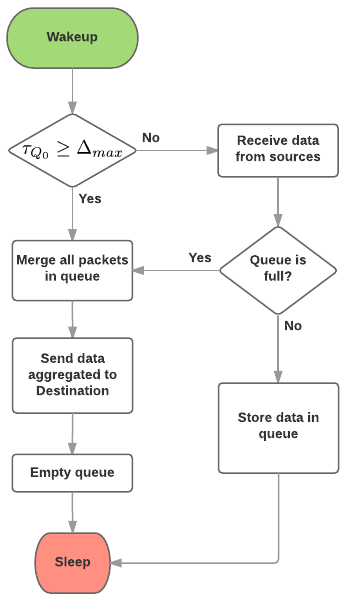
\epsfig{file = ./chapters/chapter5/images/fixed_aggregation.png}
\caption{Behavior of sensor node with Fixed Aggregation MAC protocol.}
\label{fig:fixed_aggregation}
\end{center}
\end{figure}
As other sensor nodes, the relay node uses also the technique duty cycling, it switches between sleep and awake state. But unlike the source or destination nodes, at the beginning of awake state, the relay node will decide to turn on the radio in listening state to receive data from the source nodes or in sending state to transmit the data to the next relay node or to the destination node. To avoid the packet lost caused by the queue is full, the data aggregation is higher priority than receiving data.
\subsubsection{Aggregated packet structure}
As the discussion in the section \ref{sec:fa_design} above, the relay node will aggregate all data packets in the queue and sends a big packet to the destination. A new structure of data packet is proposed in Fig.\ref{fig:aggregated_packet} below.
\begin{figure}[!b]
\begin{center}
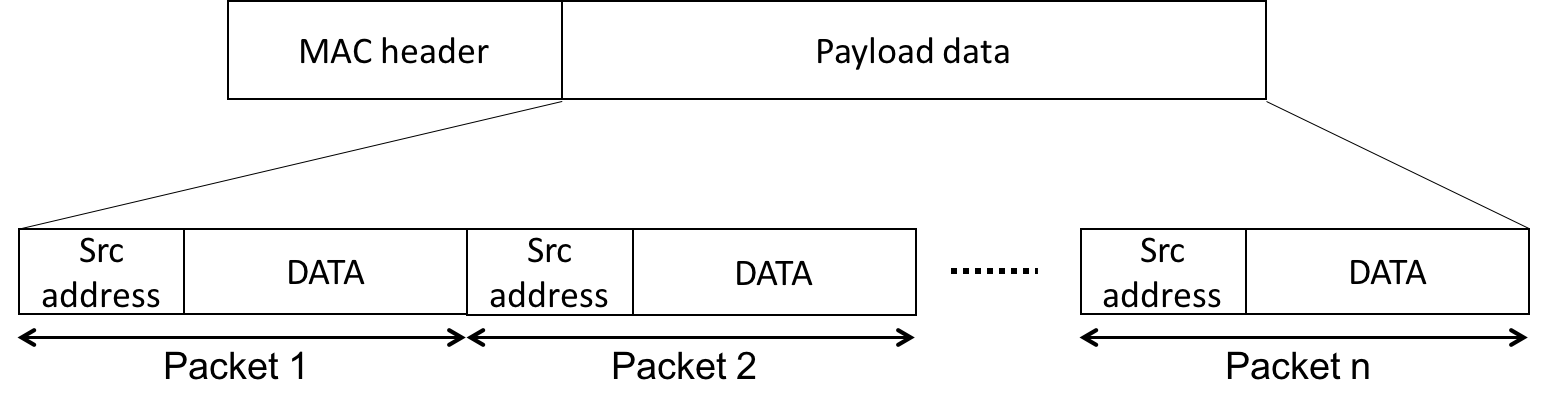
\epsfig{file = ./chapters/chapter5/images/data_structure.png, width=12cm}
\caption{New structure of aggregated packet.}
\label{fig:aggregated_packet}
\end{center}
\end{figure}
With the new structure defined, the size of aggregated data packet is dynamic and can be calculated by the equation following
\begin{equation}
l_{DATA_{agg}} = l_{DATA_{h}} + n(l_{DATA} - l_{DATA_h} + 4)
\label{eq:aggregated_data_length}
\end{equation}
\begin{equation}
t_{DATA_{agg}} = \frac{l_{DATA_{agg}} * 8}{b_{rate}}
\label{eq:aggregated_data_sent_time}
\end{equation}
where $l_{DATA}$ and $l_{DATA_h}$ is the length of data packet and its header, \textit{n} is the number of packet will be aggregated, the condition to use the new structure is \textit{n > 1}, \textit{4} is the number of byte of source address field in header (which is defined in Sec. \ref{sec:fta_frame_structure})

By applying the new structure of data packet and the energy consumption model in duty cycling \ref{sec:fta_energy_model}, the energy saved by sending a new aggregated data packet instead of many single data packet is estimated :
\begin{equation}
\begin{split}
\Delta_E &= n(E_{TX_{DATA}} + E_{RX_{DATA}}) - (E_{TX_{DATA_{agg}}} + E_{RX_{DATA_{agg}}})\\
&= n[4t_{CCA}P_{RX} + (t_{ACK} + t_{DATA})(P_{RX} + P_{TX})] \\
&\quad - [4t_{CCA}P_{RX} + (t_{ACK} + t_{DATA_{agg}})(P_{RX} + P_{TX})] \\
&= (n-1)[4t_{CCA}P_{RX} + t_{ACK}(P_{RX} + P_{TX})] + (P_{RX} + P_{TX})(nt_{DATA} - t_{DATA_{agg}})
\end{split}
\label{eq:aggregated_data_delta_energy}
\end{equation}

From the equations \ref{eq:aggregated_data_length}, \ref{eq:aggregated_data_sent_time} and \ref{eq:aggregated_data_delta_energy} we have :

\begin{equation}
\Delta_E = (n-1)[4t_{CCA}P_{RX} + t_{ACK}(P_{RX} + P_{TX})] + (P_{RX} + P_{TX})\frac{8[(n-1)l_{DATA_{h}} - 4]}{b_{rate}}
\label{eq:aggregated_data_delta_energy}
\end{equation}

The equation \ref{eq:aggregated_data_delta_energy} shows that the more packets aggregated, the more energy saved. But the length of aggregated packet is limited by the hardware of sensor node. So we can not aggregate too much data packets into one big aggregated packet. The number of packets can be aggregated is depend also on the size of data packet which is used in MAC protocol.
\subsection{Dynamic Decision Aggregation}
\subsubsection{Limitation of Fixed Aggregation}
\label{sec:limitation_fa}
In the previous section, we discussed about the Fixed Aggregation mechanism and its advantage in  saving energy consumption. An other advantage of Fixed Aggregation is that the relay nodes do not require any addition information from the source nodes. This feature allows this mechanism is implemented facilely in the MAC protocols. But the fixed waiting duration will increase unnecessarily the delay of data packet in end-to-end communication. This problem is described more detail in the Fig.\ref{fig:fixed_agg_wrong}.
\begin{figure}[!b]
\begin{center}
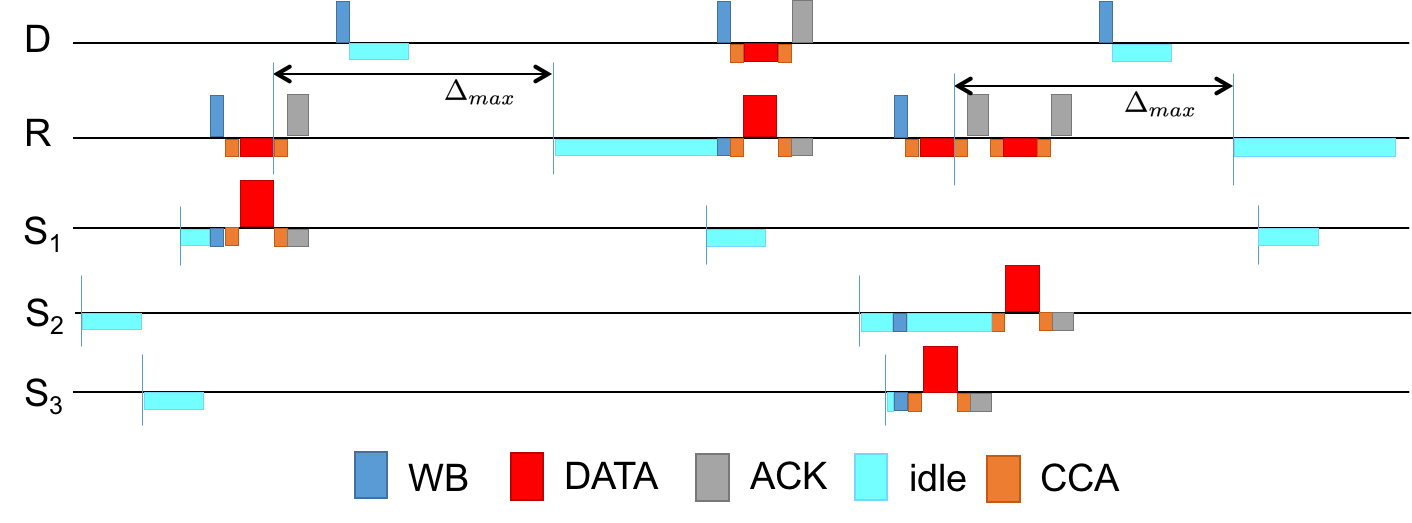
\epsfig{file = ./chapters/chapter5/images/fixed_agg_wrong.png, width=13cm}
\caption{Wasted delay time of Fixed Aggregation.}
\label{fig:fixed_agg_wrong}
\end{center}
\end{figure}
In this example, after receiving data packet from $S_1$, the relay node (\textit{R}) stores this data packet in the queue and makes a schedule to aggregate this packet with the others coming in $\Delta_{max}$ and send the big packet to the destination (\textit{D}). But within the $\Delta_{max}$ second, there is not any packet arrive so the relay node wasted the $\Delta_{max}$s. The problem is also existed in $2^{nd}$ case when the relay node receives the data packets from $S_2$ and $S_3$, it continues wait $\Delta_{max}$s after receiving the $1^{st}$ packet (from $S_3$). This waiting is wasted also.

An other limitation of Fixed Aggregation mechanism is its compatibility of integration with the MAC protocols. In some asynchronized MAC protocols (RICER \cite{ricer}, FTA-MAC \cite{fta-mac}, TAD-MAC \cite{tad-mac}) the communication of sender and receiver is initiated by the receive's WB packet. The waiting duration $\Delta_{max}$ may be caused the missing of destination's WB packet in relay node. In example shown in Fig. \ref{fig:fixed_agg_wrong}, after the waiting duration $\Delta_{max}$, the relay node wakes up and wait the WB packet from the destination, but it already missed the destination's WB packet so it must stay awake to wait the next WB packet. This problem will increase the \textit{idle listing} time and the relay node wastes the energy.
\subsubsection{Dynamic Decision Aggregation}
Dynamic Decision Aggregation is an other approach of data aggregation which avoids the problem of wasted delay time presented in Sec. \ref{sec:limitation_fa}. Unlike Fixed Aggregation mechanism, the relay node does not go to sleep after pushing the data packet into the queue, it estimates the next coming data packets. If there is one or more data packet arrive within $\Delta_{max}$ second, the relay node will wait the coming data packet to aggregate and send to the destination. But note that the duration of staying in queue of a data packet is no longer than $\Delta_{max}$, so the condition of aggregation in Dynamic Decision Aggregation is proposed in the equation following
\begin{equation}
\Delta{t_j} = \widehat{t_j} - t_c\ (\forall{j \neq i})
\label{eq:dda_delta_t_j}
\end{equation}
\begin{equation}
\Delta{t_j} \leq \Delta_{max} - \tau_{Q_0}
\label{eq:dda_condition}
\end{equation}
where \textit{i} index is the index of current source node, $\widehat{t_j}$ is the arrive time of data packet of $j^{th}$ source node, $t_c$ is the current time of system. Because the estimated time $\widehat{t_j}$ is calculated in relay node so it does not require to synchronize the system clock between the sensor nodes.
\begin{figure}[!t]
\begin{center}
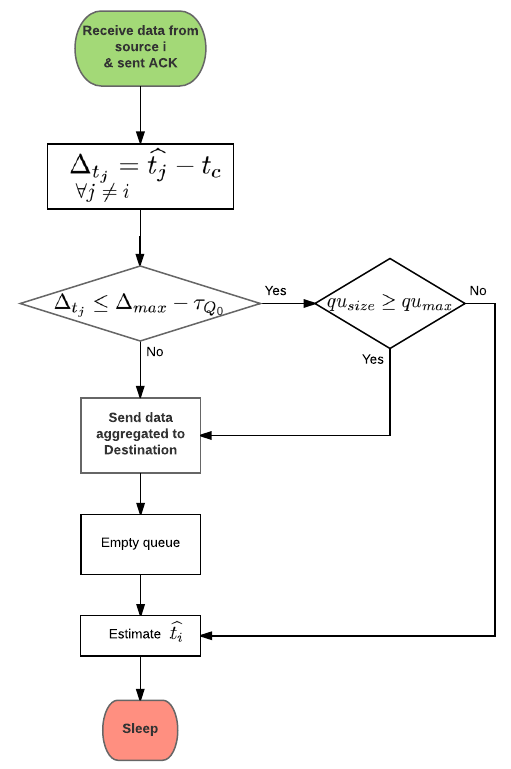
\epsfig{file = ./chapters/chapter5/images/dda.png, width=7cm}
\caption{The state machine of Dynamic Decision Aggregation mechanism.}
\label{fig:dda}
\end{center}
\end{figure}

To estimate the next coming data packet, the method of calculation is depended on the MAC protocols in which the Dynamic Decision Aggregation is implemented. These are some MAC protocols which calculated or allow to calculate easily this value such as PW-MAC \cite{pw-mac}, TAD-MAC, FTA-MAC. Almost MAC protocols do not calculate or have not any additional information which is allow to calculate the next arrival of data packet but we can estimate this value by measuring the traffic. A light weight algorithms is proposed when applying the Dynamic Decision Aggregation in RICER3 (RICER3-DDA protocol). This algorithms is presented in next section.

In considering the problem of wasted delay time presented in Sec. \ref{sec:limitation_fa}, this problem will be resolved by applying the new condition of aggregation in the equation \ref{eq:dda_condition} and \ref{eq:dda_delta_t_j} which is shown in Fig.\ref{fig:dda_2}.
\begin{figure}[!b]
\begin{center}
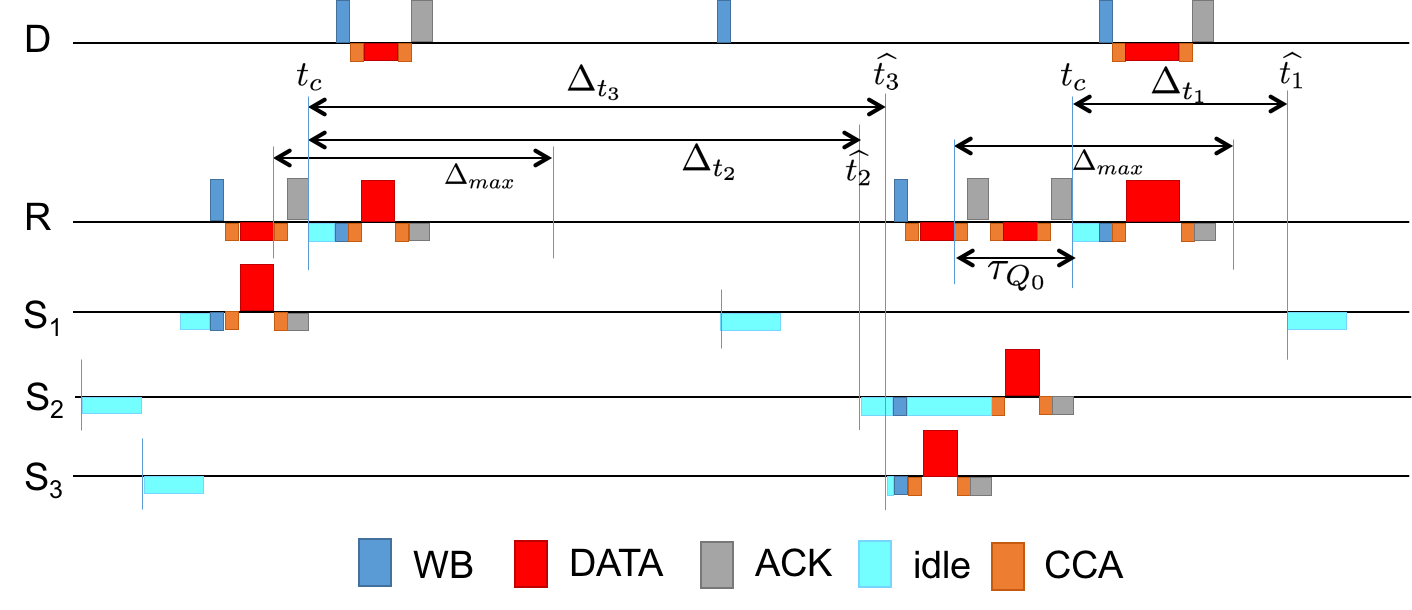
\epsfig{file = ./chapters/chapter5/images/dda_2.png, width=13cm}
\caption{Solution of wasted delay time in Dynamic Decision Aggregation mechanism.}
\label{fig:dda_2}
\end{center}
\end{figure}
Precisely, at the $1^{st}$ case, after sending the ACK packet back to $S_1$, the relay node calculates these values $\Delta_{t_2}$ \& $\Delta_{t_3}$ to make the decision of aggregation. The next arrival of data packets from $S_2$ \& $S_3$ is so long to make the aggregation so the relay node does not go to sleep, it stays awake to wait the WB from the destination and transmits the data packet to destination. In the $2^{nd}$ case, we suppose the MAC protocol already has mechanism to solve the problem of data conflict, so the process of aggregation will be started after sending the ACK packet back to $S_2$, when all communications between the relay node and the source nodes are finished. This applying will not change the algorithm of MAC protocol. 
\section{Implementation and Evaluation}
To evaluate the performance of Fixed Aggregation and Dynamic Decision Aggregation, we implement them in the exist MAC protocols like RICER3, FTA-MAC.
\subsection{Implementation of the aggregation MAC protocols in RICER3}
\subsubsection{RICER3 Fixed Aggregation (RICER3-FA)}
The implementation of Fixed Aggregation in RICER3 is applied on the relay node.
The basic behavior of RICER3-FA is described in Fig. \ref{fig:ricer_fa}. As describing in Sec. \ref{sec:fa_design}, the implementation is applied on the relay node. In each cycling, the Fixed Aggregation mechanism is executed at the end of the communication between relay node (\textit{R}) and the senders ($S_1$, $S_2$, $S_3$) to verify the aggregation condition in Eq. \ref{eq:fa_condition}. If the condition is satisfied, the relay node will stay awake to wait the \textit{WB} from the receiver and sends the aggregated data packet to the receiver. Otherwise, it go to sleep and finish a duty cycling. An additional timer is used in the relay node to compute the queuing time of the first packet. \ref{eq:dda_delta_t_j}
\begin{figure}[!b]
\begin{center}
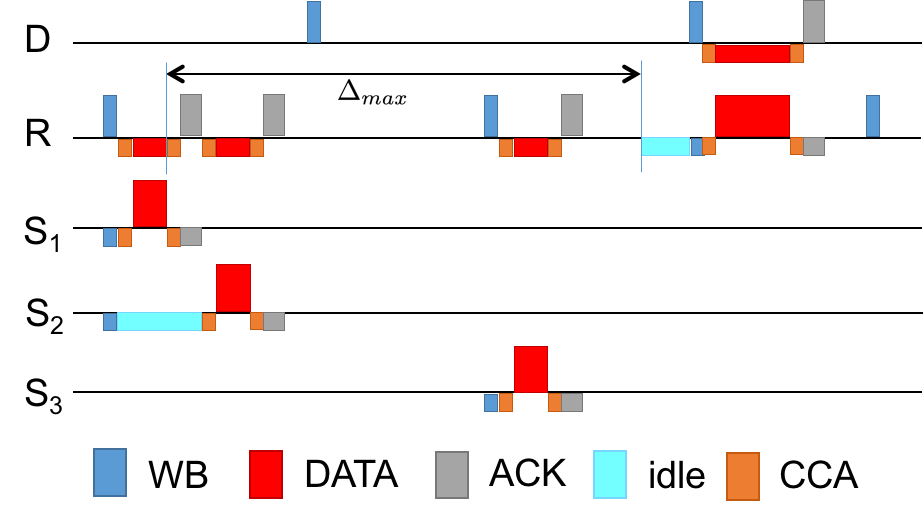
\epsfig{file = ./chapters/chapter5/images/ricer_agg.png, width=12cm}
\caption{Basic behavior of RICER with Fixed Aggregation.}
\label{fig:ricer_fa}
\end{center}
\end{figure}
\subsection{Evaluation}
\subsubsection{Simulation parameters}
\subsubsection{Results}
%\blankspace
%\input{./Chapters/Chapter6/Chapter6} % 
%\blankspace
%% Conclusion

\chapter*{Conclusion and perspectives} % Write in your own chapter title
\label{Conclusion}
\addtotoc{Conclusion and perspectives}
\lhead{\emph{Conclusion and perspectives}} % Write in your own chapter title to set the page header


 % Conclusion
%% Chapter 7

\chapter*{Personal Publications} % Write in your own chapter title
\label{Publication}
\lhead{\emph{Personal Publication}} % Write in your own chapter title to set the page header
 % Publication

%% ----------------------------------------------------------------
% Now begin the Appendices, including them as separate files


%\appendix % Cue to tell LaTeX that the following 'chapters' are Appendices

%% Appendix A

\chapter{Appendix}
\label{AppendixA}
%\lhead{Appendix A. \emph{Appendix Here}}

Write your Appendix content here.	% Appendix Title

%\input{./Appendices/AppendixB} % Appendix Title

%\input{./Appendices/AppendixC} % Appendix Title

%\addtocontents{toc}{\vspace{2em}}  % Add a gap in the Contents, for aesthetics
%\backmatter

%\addtocontents{toc}{\vspace{2em}} % Add a gap in the Contents, for aesthetics
%\blankspace

%% ----------------------------------------------------------------
%\label{Bibliography}
%\lhead{\emph{Bibliography}}  % Change the left side page header to "Bibliography"
\bibliographystyle{unsrtnat}  % Use the "unsrtnat" BibTeX style for formatting the Bibliography
%\bibliography{bibliography_precoder}  % The references (bibliography) information are stored in the file named "these.bib"
\bibliography{vanthiepnguyen}
%\blankspace
%\includepdf[offset= 85 -80]{./Chapters/last_page.pdf}
%}
\end{document}  % The End
%% ----------------------------------------------------------------